\section{Secondary Storage}

\paragraph{Secondary Storage --- structure}
\begin{itemize}
  \item hard disk drives
  \item solid state drive
  \item RAID structure
  \item tertiary storage devices (DVD, magnetic tape)
\end{itemize}

\paragraph{Hard Disk Drives --- anatomy}
\begin{itemize}
  \item stack of magnetic platters
  \item disk arms contain disk heads per recording surface, read/write to platters
  \item \textbf{storage}: \\*
    $ - $ platters divided into concentric \emph{tracks} \\*
    $ - $ \emph{cylinder}: stack of tracks of fixed radius \\*
    $ - $ tracks of fixed radius divided into \emph{sectors}
\end{itemize}

\paragraph{Flash Memory}
\begin{itemize}
  \item \textbf{advantages}: \\*
    $ - $ solid state \\*
    $ - $ lower power consumption/heat \\*
    $ - $ no mechanical seek
  \item \textbf{disadvantages}: \\*
    $ - $ limited number of overwrites \\*
    $ - $ limited durability
\end{itemize}

\paragraph{RAID}
\begin{itemize}
  \item \textbf{idea}: improve performance + reliability of storage system by storing redundant data
\end{itemize}
\begin{figure}[h]\centering\label{RAID}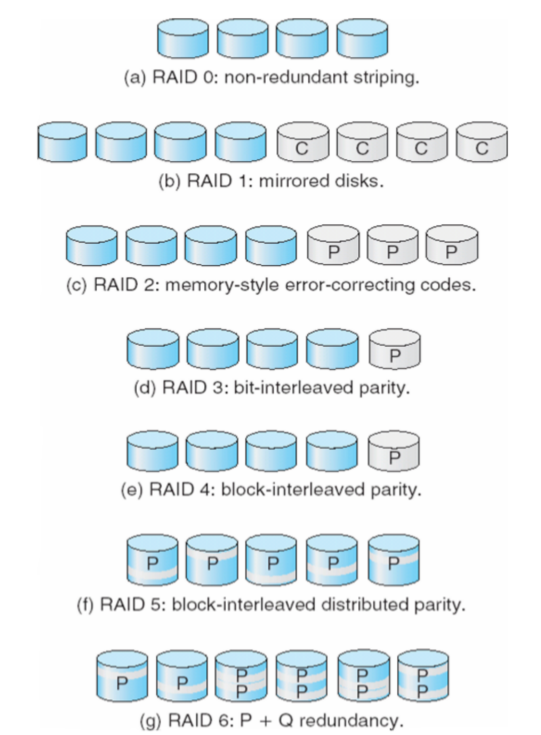
\includegraphics[width=0.2\textwidth]{RAID}\end{figure}